\section{Theorie}
\label{sec:Theorie}

\subsection{Interferenz, Intensität und die Notwendigkeit kohärenten Lichts}

Für die Beschreibung der physikalischen Vorgänge wird das Wellenmodell des Lichts verwendet. 
Dies beschreibt Licht als eine in Richtung des Wellenvektors $\vec{k}$ propagierende elektromagnetische Welle
\begin{equation*}
    \vec{E}=\vec{E}_0 \symup{e}^{\symup{i}(\vec{k}\cdot \vec{r}-\omega t +\delta)}\,,
\end{equation*} 
deren Intensität beim Auftreffen auf eine Fläche gemessen werden kann. 
Diese ist proportional zum Amplitudenquadrat
\begin{equation*}
    I \propto |\vec{E}|^2
\end{equation*}
und somit bei einer einzelnen Wellenfunktion konstant. 
Werden zwei Lichtwellen derselben Frequenz $\omega$ und desselben Wellenvektors $\vec{k}$ überlagert, hängt die Intensität 
von den Phasenverschiebungen $\delta_1$ und $\delta_2$ ab: 
\begin{equation*}
    I \propto 1+\cos (\delta_2-\delta_1)\,.
\end{equation*}
Je nach Phasenlage kann sie sich deshalb sogar ganz auslöschen und es sollten deutliche Interferenzerscheinungen sichtbar sein, wenn 
das Licht zweier Lichtquellen überlagert wird. 

Nun muss jedoch die Entstehung des Lichts bei konventionellen Lichtquellen berücksichtigt werden. 
Dies entsteht für gewöhnlich durch die Emission eines Wellenpakets mit einer Frequenz im optischen Bereich, wenn ein Elektron 
eines angeregten Atoms wieder in den Grundzustand zurückkehrt. 
Da die Emissionen und Anregungen der Atome in der Zeit statisch verteilt sind, emittieren die Atome derselben Quelle zu unterschiedlichen Zeiten die 
räumlich begrenzten Wellenpakete.
Dies führt dazu, dass die Differenz $\delta_2-\delta_1$ stark mit der Zeit schwankt und sich somit der Interferenzterm $\cos (\delta_2-\delta_1$ 
über den Messzeitraum auslöscht. 
Konventionelle Lichtquellen stellen somit kein für das Experiment brauchbares kohärenztes Licht zur Verfügung. 
Deshalb werden Laser -- light amplification by stimulated emission of radiation -- verwendet, deren Atome durch 
stimulierte Emission Licht derselben Phasendifferenz $\delta$ aussenden. 

Zur Veranschaulichung des Begriffs der Kohärenzlänge kann Abbildung \ref{fig:Prinzip} betrachtet werden. 
\begin{figure}
    \centering
    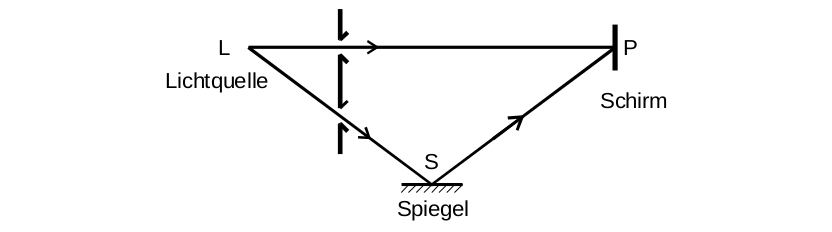
\includegraphics[width=\textwidth]{plots/Interferenz_Prinzip.png}
    \caption{Möglichkeit zur Erzeugung von Interferenzerscheinungen.}
    \label{fig:Prinzip}
\end{figure}
Dort wird Licht desselben Entstehungsorts -- also derselben Phasenlage $\delta$ und Amplitude $\vec{E}_0$ -- mittels eines 
Strahlteilers geteilt und auf zwei verschiedenen Wegen mittels Reflexion an einem Spiegel am Punkt P wieder zusammengebracht. 
Durch den (messbaren) Wegunterschied $\Delta$ entsteht eine feste Phasendifferenz, die sich in entsprechender Interferenz zeigen sollte. 
Konstruktive Interferenz, also die maximal mögliche Intensität, ist bei ganzzahligen Vielfachen der Wellenlänge $\lambda$ möglich 
\begin{equation*}
    \Delta = n\lambda \,, \, n \in \mathbb{N}
\end{equation*}
und vollständige Auslöschung, also destruktive Interferenz, bei ungeradzahligen Vielfachen der halben Wellenlänge:
\begin{equation*}
    \Delta = (2n+1)\frac{\lambda}{2}\,,\,n\in\mathbb{N}\,.
\end{equation*}
Ist der Wegunterschied $\Delta$ jedoch zu groß gewählt und übersteigt die Länge der emittierten Wellengruppe, treffen 
die Teilstrahlen nacheinander am Schirm auf und es ist keine Interferenz messbar, sondern nur die Intensität der einzelnen 
Strahlen. 
Der angesichts dieser Umstände maximal mögliche Wegunterschied wird die Kohärenzlänge $l$ einer Lichtquelle genannt. 
Analytisch kann diese über 
\begin{equation*}
    l=N\lambda
\end{equation*}
formuliert werden, wobei $N$ die maximal mögliche Anzahl der Interferenzmaxima darstellt. 

\subsection{Das Michelson-Interferometer}

In Abbildung \ref{fig:Aufbau_Interf} ist der schematische Aufbau eines Michelson-Interferometers zu sehen. 
\begin{figure}
    \centering
    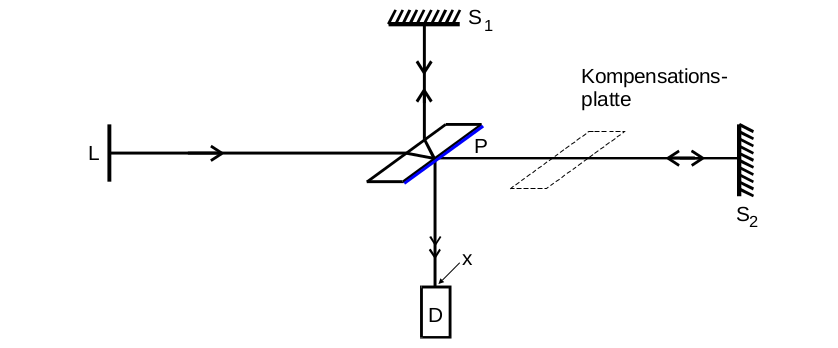
\includegraphics[width=\textwidth]{plots/Aufbau_Interf.png}
    \caption{Prinzipieller Aufbau eines Interferometers.}
    \label{fig:Aufbau_Interf}
\end{figure}
Der von der Lichtquelle L ausgehende Lichtstrahl wird mittels beispielsweise einer semipermeablen Platte P in zwei Strahlen aufgeteilt, 
welche nach Reflexion an den Spiegeln $\symup{S}_1$ und $\symup{S}_2$ am Detektor D wieder auftreffen. 
Diese sind kohärent, sofern ihr optischer Weglängenunterschied kleiner als ihre die Kohärenzlänge ist. 
Zwischen P und $\symup{S}_2$ befindet sich eine Kompensationsplatte mit dem gleichen Brechindex wie die semipermeable Platte.
So wird der sonst entstehende Wegunterschied durch das Durchlaufen von Materie mit unterschiedlichen Brechindizes (die beiden 
Strahlen durchlaufen P unterschiedlich oft) eliminert. 

Um die Wellenlänge zu messen, kann die Verschiebung des Interferenzmusters genutzt werden, die auftritt, wenn ein Spiegel um $\Delta d$ verändert wird. 
Dies lässt sich über (o.B.d.A. sei $\vec{k} \parallel \vec{e}_x$) 
\begin{align*}
    I &\propto |E_0|^2 (\symup{e}^{\symup{i}(kx)}+\symup{e}^{\symup{i}(k(x+2\Delta d + \symup{\pi}))}(\symup{e}^{-\symup{i}(kx)}+\symup{e}^{-\symup{i}(k(x+2\Delta d + \symup{\pi}))})) \\
      &= 2|E_0|^2(1+\cos (2k \Delta d + \symup{\pi}))
\end{align*}
erklären, wobei berücksichtigt wird, dass bei der Reflexion an P eine zusätzliche Phasenverschiebung von $\symup{\pi}$ hinzukommt. 
Mit $k=\sfrac{2\symup{\pi}}{\lambda}$ ist ersichtlich, dass die Interferenzmaxima in Abständen von $\sfrac{\lambda}{2}$ auftreten. 
Wird nun mithilfe einer hinreichend präzisen Mikrometerschraube ein Spiegel um eine entsprechende Differenz $\Delta d$
verschoben und wird die Anzahl $z\gg 1$ der vorbeiziehenden Interferenzmaxima gezählt, kann die Wellenlänge über 
\begin{equation*}
    \Delta d=z \cdot \frac{\lambda}{2}
\end{equation*}
bestimmt werden. 

Eine Möglichkeit, Brechindexunterschiede zu messen, eröffnet sich mithilfe des in Abbildung \ref{fig:Brechindex_messen} 
dargestellten Aufbaus. 
\begin{figure}
    \centering
    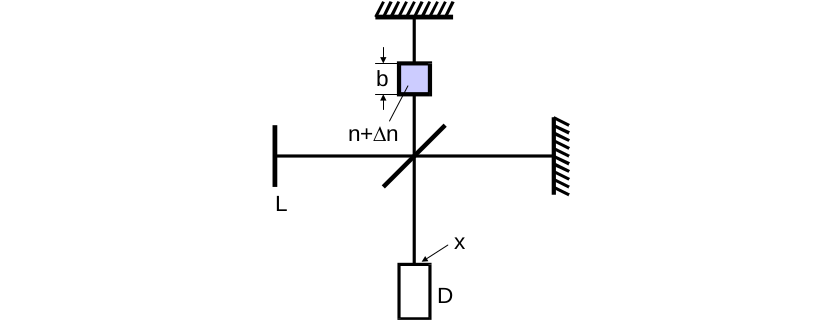
\includegraphics[width=\textwidth]{plots/Brechindex_messen.png}
    \caption{Eine Möglichkeit, mithilfe des Interferometers Brechindexunterschiede zu messen.}
    \label{fig:Brechindex_messen}
\end{figure}
Dort wird eine Probe des entsprechenden Mediums mit Länge $b$ in einen der beiden Strahlgänge gehalten, der Brechindex 
im Vergleich zur Umgebung mit Brechindex $n$ betrage $n+\Delta n$.
Der optische Weglängenunterschied beträgt dann $b\cdot \delta n$ und mit bekannter Wellenlänge kann der Brechindexunterschied 
bequem über 
\begin{equation}
    b\cdot \Delta n=z\cdot \frac{\lambda}{2}
    \label{eqn:b}
\end{equation}
ermittelt werden. 
Da im Allgemeinen $\lambda \ll b$ gilt, können mit dieser Methode gut Brechindexunterschiede der Größenordnung von etwa $\num{e-5}$ gemessen werden. 
